% !TeX spellcheck = de_DE
\section{Neuronale Netze}
\label{sec:neuroal_networks}
Klassische Algorithmen in der Informatik beschreiben, mit welchen Schritten ein spezielles Problem gelöst werden kann. In vielen Anwendungsfällen, wie zum Beispiel beim Sortieren einer Liste, verwenden Computersysteme diese und lösen das gegebene Problem schneller und effizienter als es Menschen möglich ist. 
% DODO RELATIVIERUNG! Nicht: Es gibt keine Algorithmen, sondern: Es ist schwierig welche zu finden
Dennoch gibt es Aufgaben, die von Menschen ohne Aufwand gelöst werden, aber Computersysteme vor große Herausforderungen stellen. Hierzu zählt unter anderem die Klassifizierung von Bildern. Ein Mensch kann zum Beispiel Bilder von Hunden und Katzen unabhängig von Blickwinkel und Bildqualität unterscheiden beziehungsweise richtig zuordnen. Trotzdem lassen sich für solche Probleme keine klassischen Algorithmen finden, da die Lösung von vielen subtilen Faktoren abhängig ist \cite{kriesel2008kleiner}.

In vielen dieser Aufgabenfelder werden \ac{KNN} eingesetzt, welche von biologischen neuronalen Netzen inspiriert sind und zum Forschungsgebiet des maschinellen Lernens gehören. Auch wenn die \ac{KNN} heute aktuell sind und viel Aufmerksamkeit erhalten, ist die Grundlage die Arbeit von \citeauthor{mcculloch1943logical}, welche 1943 ein einfaches neuronales Netz mit Schwellwerten entwickelt haben. Dies ermöglicht die Berechnung von logischen und arithmetischen Funktionen \cite{mcculloch1943logical}. In den folgenden Jahrzehnten wurde die Funktionsweise der neuronalen Netze weiterentwickelt und der Einsatz in verschieden Aufgabenfeldern ermöglicht. Hierzu zählen neben der Klassifizierung von Bildern \cite{krizhevsky2012imagenet} unter anderem das Erkennen und die Interpretation von Sprache \cite{hinton2012deep}, \cite{andor2016globally} sowie das selbständiges Lösen von Computer- und Gesellschaftsspielen \cite{mnih2013playing}, \cite{silver2016mastering}. 

In diesem Kapitel wird zuerst ...
\subsection{Biologische neuronale Netze}
\label{subsec:biological_neuraL_networks}
Wie bereits beschrieben, orientiert sich das Fachgebiet der \ac{KNN} an den erfolgreichen biologischen neuronalen Netzen, wie zum Beispiel dem menschlichen Gehirn \cite{kriesel2008kleiner}. In diesem Abschnitt werden die Eigenschaften betrachtet, die das Vorbild erfolgreich machen und für die \ac{KNN} übernommen werden sollen. Im Zuge dessen wird ein grober Überblick über die Struktur und Funktionsweise des menschlichen Gehirns gegeben. 
\\\\
Jede Sekunde erfassen die Rezeptoren des menschlichen Körpers unzählige Reize, wie zum Beispiel Licht, Druck, Temperatur und Töne. Die Reize werden anschließend elektrisch oder chemisch kodiert und über Nervenbahnen an das Gehirn geleitet, welches die Aufgabe hat, diese zu filtern, zu verarbeiten und entsprechend zu reagieren. Als Reaktion können zum Beispiel Signale an entsprechende Muskeln oder Drüsen gesendet werden \cite{kinnebrock2018neuronale}. 

Bevor im nächsten Kapitel die Funktionsweise des Gehirns näher betrachtet wird, werden hier zunächst drei Eigenschaften beschrieben, die klassische Algorithmen entweder nicht besitzen oder nur schwer umsetzen können, aber für biologische neuronale Netze keine Herausforderung sind. Ziel ist es, diese mit den \ac{KNN} umzusetzen \cite{kriesel2008kleiner}.
\begin{enumerate}
	\item \textbf{ Fähigkeit zu Lernen} \\
	Das menschliche Gehirn ist nicht wie ein klassischer Algorithmus für seine Aufgaben programmiert. Stattdessen besitzt es die Fähigkeit, durch Nachahmen oder Ausprobieren zu lernen \cite{kriesel2008kleiner}. Dafür wird das angestrebte Ergebnis mit dem tatsächlich erzielten verglichen und das Verhalten entsprechend angepasst. Dies ermöglicht es Menschen, verschiedene Aufgabengebiete erfolgreich zu lösen und sich ändernden Anforderungen anzupassen.
	
	\item \textbf{Fähigkeit zur Generalisierung}\\
	Allerdings kann nicht jedes mögliche Szenario für ein Aufgabenfeld durch Ausprobieren oder Beobachtung gelernt werden. Trotzdem trifft das Gehirn in den meisten Situationen plausible Lösungen, da es die Fähigkeit zur Generalisierung besitzt 
	\cite{kriesel2008kleiner}. Das bedeutet, dass viele Situationen bereits bekannten Problemen zugeordnet werden können, mithilfe derer eine passende Verhaltensstrategie ausgewählt wird. 
	
	\item \textbf{Toleranz gegenüber Fehlern}\\
	Die Fähigkeit zu Generalisieren erlaubt auch eine hohe Fehlertoleranz gegenüber verrauschten Daten. Bei oben genanntem Beispiel der Klassifizierung von Bildern kann ein Teil des Bildes fehlen oder unscharf sein, trotzdem kann das abgebildete Motiv richtig zugeordnet werden.
\end{enumerate}

\subsubsection{Struktur des menschlichen Gehirns}
Das Forschungsgebiet der Neurowissenschaften befasst sich unter anderem mit dem menschlichen Gehirn, dessen Funktionsweise auch heute noch nicht vollständig erforscht ist. Dennoch ist schon seit 1861 durch die Arbeit von Paul Broca bekannt, dass es im menschlichen Gehirn verschiedene Regionen mit unterschiedlichen Aufgaben gibt \cite{russell2013kunstliche}. Zum Beispiel wird das sogenannte Kleinhirn (Cerebellum) für einen Großteil der motorischen Koordination verwendet, während an das Großhirn (Telencephalon) unter anderem visuelle Reize geleitet werden \cite{kriesel2008kleiner}. Trotz der unterschiedlichen Aufgaben haben alle Bereiche des Gehirns einen gemeinsamen Grundbaustein, die sogenannten Neuronen \cite{russell2013kunstliche}. Im Folgenden wird der Aufbau und die Funktionsweise von diesen oberflächlich im Bezug zu den später vorgestellten künstlichen Neuronen betrachtet. Für einen vollständigen Überblick und eine genaue Beschreibung der Vorgänge wird auf entsprechende Fachliteratur verwiesen.\\
%TODO Fachliteratur LINK
\begin{figure}[h]
	\centering
	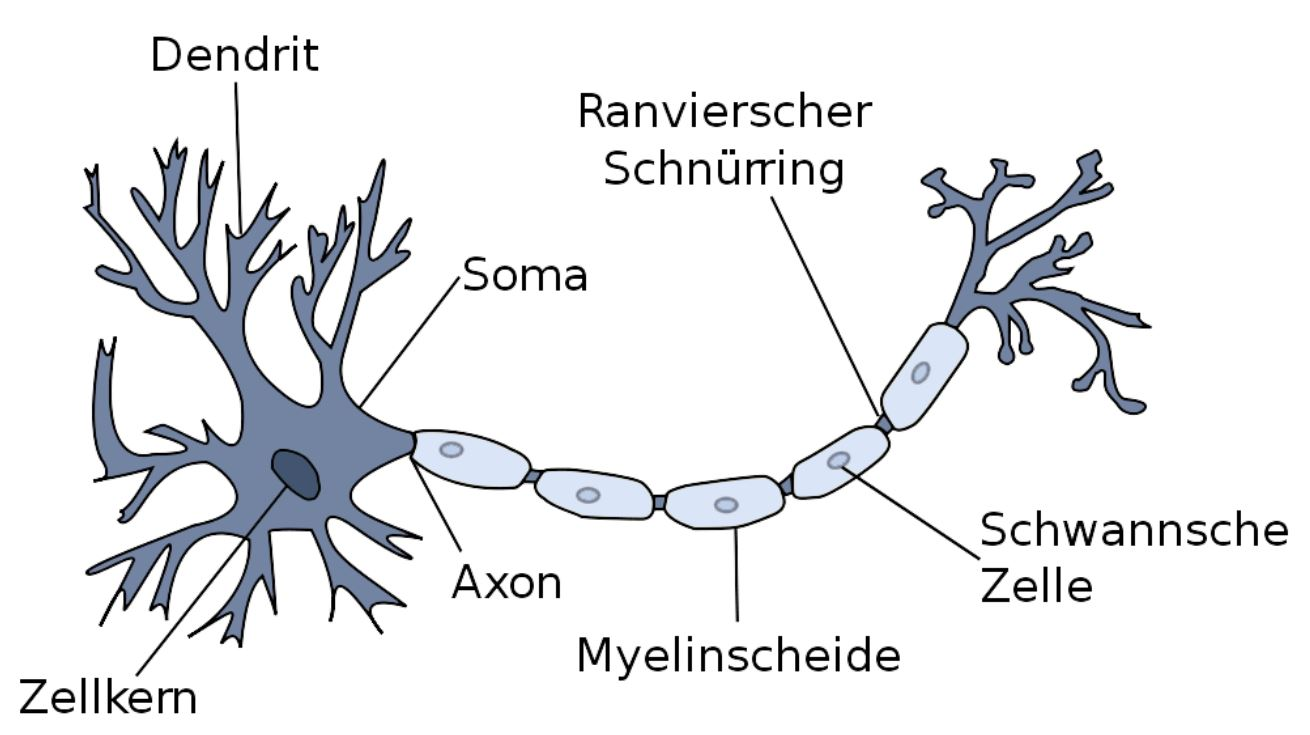
\includegraphics[width=0.75\textwidth]{./img/biologial_neuron.JPG} 
	\caption{Schematische Abbildung einer Nervenzelle, Quelle \cite{kriesel2008kleiner}.}
	\label{fig:biological_neuron}
\end{figure}
Das menschliche Gehirn besitzt ungefähr ${10}^{11}$ einzelne Neuronen, deren schematischer Aufbau in \autoref{fig:biological_neuron} dargestellt ist. Jedes Neuron besitzt einen Zellkern, der sich im Zellkörper (Soma) befindet. Von dem Zellkörper gehen mehrere Fasern aus, die Dendriten genannt werden \cite{russell2013kunstliche}. An diesen befinden sich Synapsen, welche als Übertragungsstelle fungieren und elektrische oder chemische Signale von Rezeptoren oder anderen Neuronen empfangen \cite{kriesel2008kleiner}. Typischerweise empfängt ein Neuron Signale von 2000 bis 10.000 anderen Nervenzellen \cite{zell2003simulation}. \\
Synapsen, die elektrische Signale empfangen, haben eine starke, direkte, nicht regulierbare Verbindung vom Sender zum Empfänger. Diese sind für hart kodierte Verhaltensmechanismen nützlich, wie zum Beispiel den Fluchtreflex. Die chemische Synapse hingegen ist nicht direkt mit dem Sender verbunden, sondern durch den synaptischen Spalt getrennt \cite{kriesel2008kleiner}. Zur Übertragung eines elektrischen Signals wird dieses auf der präsynaptischen Seite in ein chemisches Signal kodiert, indem Neutransmitter freigesetzt werden. Diese können über den synaptischen Spalt übertragen und anschließend auf der postsynaptischen Seite wieder in ein elektrisches Signal kodiert werden. Ein großer Vorteil dieser Übertragungsart ist die Regulierbarkeit \cite{kriesel2008kleiner}. Verschiedene Neurotransmitter können unterschiedliche Effekte auf das Neuron haben, beispielsweise anregend (exzitatorisch) oder hemmend (inhibitorisch) \cite{kirschbaum2008biopsychologie}. Zusätzlich kann die Menge der freigesetzten Neurotransmitter die Stärke des Signals beeinflussen \cite{kriesel2008kleiner}. Langfristig gesehen können auch neue Verbindungen entstehen oder alte aufgelöst werden. Es wird angenommen, dass dies die Grundlage des Lernens im menschlichen Gehirn ist \cite{russell2013kunstliche}.\\
Sowohl die erregenden als auch hemmenden Signale werden über die Dendriten an den Axonhügel weitergeleitet, welcher sich zwischen dem Soma und dem Axon befindet. Dort werden die Signale akkumuliert. Wird bei diesem Vorgang ein gewisser Schwellwert überschritten, wird ein elektrischer Impuls erzeugt, der über das Axon weitergeleitet wird \cite{kirschbaum2008biopsychologie}. Das Axon ist typischerweise 1cm, in Ausnahmen sogar bis zu einem 1m lang und wird von der Myelinscheide umgeben, die unter anderem Schutz vor mechanischer Überbeanspruchung bietet \cite{russell2013kunstliche}. Zusammen mit den Ranvierschen Schnürringen  ermöglicht diese zudem eine schnellere Weiterleitung des Aktionspotenzials \cite{kirschbaum2008biopsychologie}. Das Axon endet mit dem sogenannten Endknopf, auch Axonterminal genannt. Dieses ist mit den Synapsen von anderen Neuronen verbunden und setzt beim Eintreffen eines Signals die Neurotransmitter frei und überträgt somit das Signal \cite{kirschbaum2008biopsychologie}. Typischerweise gibt ein einzelnes Neuron sein Signal an 1000 bis 10.000 anderen Neuronen weiter, in Extremfällen sogar an bis zu 150.000 andere Neuronen \cite{zell2003simulation}, die alle parallel arbeiten. So entsteht ein sehr großes und leistungsfähiges neuronales Netz. 

\subsection{Künstliche neuronale Netze}
\ac{KNN} sind ein mathematisches Modell, das im Vergleich zum biologischen Vorbild stark vereinfacht und idealisiert ist. Trotzdem können unterschiedliche mathematische Funktionen abgebildet werden. In diesem Kapitel werden die grundsätzliche Funktionsweise sowie die einzelnen Komponenten der \ac{KNN} vorgestellt. \\\\
% TODO ABBILDUNG!!!
Betrachtet man ein \ac{KNN} als Blackbox (TODO REFERENZ BILD), gibt es eine Menge an Eingabewerten, die in einem Eingabevektor kodiert sind und eine Menge an Ausgaben, die in einem Ausgabevektor kodiert sind \cite{scherer2013neuronale}. Die Eingaben werden im Falle der \ac{KNN} nicht durch Rezeptoren erfasst sondern durch ein Optimierungsproblem gegeben. Der Ausgabevektor soll das gewünschte Ergebnis enthalten. Die Interpretation von diesem variiert je nach Optimierungsproblem und Netzarchitektur. \\

Betrachtet man die Struktur der \ac{KNN} sind einige Ähnlichkeiten zum biologischen Vorbild erkennbar. Diese werden im folgenden genauer betrachtet \cite{zell2003simulation}:
\begin{enumerate}
	\item \textbf{Neuronen}\\
	Ähnlich zu den biologischen neuronalen Netzen, besteht auch das \ac{KNN} aus vielen Neuronen \cite{zell2003simulation}. Dies sind einfache Recheneinheiten, die primitive Funktionen bestimmen können \cite{scherer2013neuronale} und deren genaue Funktionsweise in Kapitel \ref{subsec:neuron} erläutert wird. Vorweggenommen sei, dass ein Neuron mehrere Eingabewerte besitzt, welche gewichtet sind und akkumuliert werden. Hierbei entsteht ein skalarer Ausgabewert, der den Aktivierungsgrad des Neurons repräsentiert und von anderen Neuronen als Eingabe verwendet werden kann \cite{kriesel2008kleiner}. 
	 
	\item \textbf{Gerichtete gewichtete Verbindungen}\\
	Wie im vorherigen Punkt angedeutet, sind Neuronen über gerichtete Verbindungen miteinander vernetzt. Der Aktivierungszustand eines Neurons wird entsprechend der Verbindungen an die Zielneuronen weitergegeben, welche diesen Wert als Eingabe verarbeiten. Wie bei den biologischen neuronalen Netzen auch, können Eingaben unterschiedlich stark anregend und hemmend wirken. Dies wird bei den \ac{KNN} über Gewichte in den Verbindungen realisiert \cite{zell2003simulation}.
	
	\item \textbf{Struktur und Gewichte}\\
	Der Ausgabevektor eines \ac{KNN} ist abhängig von der Struktur des Netzwerkes und der Gewichte in den einzelnen Verbindungen.
	Für das erfolgreiche Lösen eines Optimierungsproblems muss ein \ac{KNN} die richtige Kombination aus Neuronen, Netzwerkstruktur und gewichteten Verbindungen besitzen. Diese müssen durch Lernverfahren bestimmt werden, auf die in Kapitel \ref{subsec:optimization_strategies} näher eingegangen wird.
\end{enumerate}
Trotz der vorgestellten Ähnlichkeiten gibt es sehr viele Unterschiede zwischen den biologischen neuronalen Netzen und den \ac{KNN}. Beispiel hierfür ist der Größenunterschied. Das menschlichge Gehirn mit seinen ${10}^{11}$ Neuronen besitzt pro Neuron ungefähr $10^4$ Verbindungen, während die meisten \ac{KNN} nur ${10}^{2}$ bis ${10}^{4}$ Neuronen mit insgesamt ${10}^{5}$ Verbindungen besitzen. Auch werden keine chemischen Effekte, die auf benachbarte Neuronen wirken, sowie zeitliche und räumliche Lokalitätsprinzipien beachtet \cite{zell2003simulation}. Aus diesen Gründen sind die \ac{KNN} keine Nachbildung der biologischen neuronalen Netzen sondern verwenden diese nur als Inspiration. 

\subsection{Das Neuron}
\label{subsec:neuron}
% TODO ABBILDUNG
In diesem Kapitel wird die Funktionsweise der einzelnen Neuronen betrachtet. Hierfür werden drei Phasen vorgestellt, in denen die Ausgabe eines einzelnen Neurons berechnet wird. Betrachtet man ein \ac{KNN}, führen typischerweise mehrere Verbindungen zu einem Neuron $j$, welche von den Neuronen $i_1, i_2, ..., i_n$ ausgehen \cite{kriesel2008kleiner}. Dieses ist schematisch in Abbildung (TODO ABBILDUNG EINFÜGEN) dargestellt.

\subsubsection{Propagierungsfunktion} 
Die Ausgabewerte $o_{i_1}, o_{i_2}, ..., o_{i_n}$ der Neuronen $i_1, i_2, ..., i_n$ werden als Eingabewerte für das Neuron $j$ verwendet. Für jeden Eingabewert existiert ein entsprechendes Gewicht $w_1, w_2, ..., w_n$ \cite{kriesel2008kleiner}. Somit repräsentiert $w_{ij}$ das Gewicht für die Verbindung von Neuron $i$ zu Neuron $j$ \cite{zell2003simulation}. Die Propagierungsfunktion $f_{prop}$ berechnet die Netzeingabe $net_j$, welche in der nächsten Phase weiterverwendet wird \cite{kriesel2008kleiner}. 
$$net_j=f_{prop}(o_1, o_2, ..., o_n, i_1, i_2, ..., i_n)$$
Die meist verwendete Propagierungsfunktion, welche auch in den späteren Beispielen genutzt wird, ist die gewichtete Summe. Hierbei werden, entsprechend der Formel, die Werte $o_i$ mit dem entsprechenden Gewicht $w_i$ multipliziert und aufsummiert \cite{kriesel2008kleiner}:
$$net_j=\sum_{i}(o_{i} \cdot w_{i, j})$$
% TODO eventuell produkt einfügen?

\subsubsection{Aktivierungsfunktion}
\label{subsubsec:activatoin_function}
Der Aktivierungszustand $a_j(t)$ gibt den Grad der Aktivierung von Neuron $j$ zum Zeitpunkt $t$ an \cite{zell2003simulation}. Ein neuer Aktivierungszustand zum Zeitpunkt $t+1$ wird mit der Aktivierungsfunktion $f_{act}$ berechnet. Diese berücksichtigt nicht nur die Netzeingabe $net_j(t)$ sondern auch den vorherigen Aktivierungszustand $a_j(t)$ und den Schwellwert $\Theta$ der Aktivierungsfunktion \cite{zell2003simulation}. Ein Schwellwert $\Theta_j$, auch Bias genannt, ist dem Neuron $j$ zugeordnet und gibt die Stelle an, an welcher die Aktivierungsfunktion die größte Steigung hat \cite{kriesel2008kleiner}. Somit kann die Berechnung der Aktivierung $a_j(t+1)$ durch folgende Formel ausgedrückt werden \cite{zell2003simulation}:
$$a_j(t+1)=f_{act}(a_j(t), net_j, \Theta_j)$$
Bei der Berechnung kommt dem Schwellwert $\Theta$ eine besondere Bedeutung zu. Oftmals verwenden einige oder alle Neuronen eines \ac{KNN} dieselbe Aktivierungsfunktion, die Schwellwerte hingegen unterscheiden sich je nach Neuron. Des Weiteren sei angemerkt, dass  die vorherige Aktivierung $a_j(t)$ je nach Netzstruktur oft nicht bei der Berechnung berücksichtigt wird \cite{kriesel2008kleiner}. Zudem wird in der Praxis bei Verwendung der gewichteten Summe als Propagierungsfunktion der Schwellwert eines Neurons oft schon in der ersten Phase miteinbezogen. Hierdurch ändert sich die Berechnung der Netzeingabe zu $net_j=\sum_{i}(o_{i} \cdot w_{i, j}) - \Theta_j$. Bei der Berechnung der Aktivierungsfunktion gilt dann $\Theta_j = 0$.
\\\\
% TODO Abbildung
Je nach Anwendungsgebiet können verschiedene Aktivierungsfunktionen mit unterschiedlichen Eigenschaften eingesetzt werden, von denen vier in Abbildung (TODO ABBILDUNG) dargestellt sind. Im Folgenden wird angenommen, dass $\Theta_j=0$ ist.\\
Das einfachste Beispiel für eine Aktivierungsfunktion ist die sogenannte binäre Schwellwertfunktion, welche abhängig vom Schwellwert $\Theta$ nur die Werte $0$ und $1$ zurückgeben kann \cite{kriesel2008kleiner}. Die Formel hierfür ist: 
$$
f_{act}(net_j)=\left\{\begin{array}{ll}
1 & \text { wenn } net_j \geq 0 \\
0 & \text { wenn } net_j < 0
\end{array}\right.
$$
% TODO Check if really introduced Backpropagation algorithmen
Allerdings ist für diese Funktion der Wert der Ableitung immer $0$ außer an dem Schwellwert, an welchem sie nicht differenzierbar ist \cite{kriesel2008kleiner}. Diese Eigenschaften machen sie ungeeignet für bestimmte Lernverfahren, wie zum Beispiel den Backpropagation Algorithmus, auf den in Kapitel \ref{subsec:optimization_strategies} kurz eingegangen wird \cite{kriesel2008kleiner}. \\
Dieses Problem kann durch die Verwendung einer Sigmoidfunktion gelöst werden. Zwei bekannte Beispiele für Sigmoidfunktionen sind die logistische Funktion und der \ac{tanh} \cite{lecun2012efficient}. Die logistische Funktion kann Werte von 0 bis 1 annehmen und durch einen entsprechenden Parameter $T$ bezüglich der x-Achse gestreckt und gestaucht werden \cite{kriesel2008kleiner}. Berechnet wird sie mit:
% TODO check if correct T position
$$f_{act}(net_j)=\frac{1}{1+e^{-T\cdot net_j}}$$
Allerdings können neuronale Netze je nach Verfahren schneller optimiert werden, wenn das durchschnittliche Gewicht aller Verbindungen nahe 0 ist. In diesem Fall ist die \ac{tanh} Funktion besser geeignet, da sie Werte zwischen -1 und 1 annehmen kann  \cite{lecun2012efficient}. Das letzte hier vorgestellte Beispiel ist die sogenannte \emph{Rectifier} Funktion. Diese wird oft in Zusammenhang mit dem Backpropagation Algorithmus erfolgreich eingesetzt und erzielt mit diesem schneller bessere Optimierungsergebnisse \cite{glorot2011deep}. Berechnet wird sie mit:
$$f_{act}(net_j)= max(0, net_j)$$

\subsubsection{Ausgabefunktion}
Die Ausgabefunktion $f_{out}$ berechnet die Ausgabe $o_j$ von Neuron $j$. Als Eingabewert wird die Aktivierung $a_j$ verwendet \cite{zell2003simulation}. Somit ist die Funktion definiert mit:
$$o_j = f_{out}(a_j)$$
Ähnlich wie die Aktivierungsfunktion ist die Ausgabefunktion in der Praxis meistens global für alle Neuronen definiert. Zudem wird oft die Identitätsfunktion verwendet. In diesem Fall gilt $o_j = a_j$ \cite{kriesel2008kleiner}. Dies gilt auch für die später vorgestellten Beispiele. Ist die Ausgabe $o_j$ berechnet, kann sie als Eingabewert für andere verbundene Neuronen dienen.

\subsection{Netzstrukturen}
\label{subsec:network_structures}
Aus dem vorherigen Kapitel ist dargestellt, dass die Gewichte einen großen Einfluss auf das Ergebnis eines einzelnen Neurons haben. Der Ausgabevektor eines \ac{KNN} wird neben den Gewichten auch von der Anzahl an Neuronen sowie deren Verbindungsstruktur beeinflusst. Je nach Optimierungsproblem können unterschiedliche Varianten eingesetzt werden, welche in diesem Kapitel genauer vorgestellt werden. 
\\\\ % TODO ABBILDUNG
Typischerweise besitzt jedes \ac{KNN} Eingabe- und Ausgabeneuronen. Optional kann ein \ac{KNN} beliebig viele verdeckte Neuronen enthalten. Diese werden auch als \emph{Input}-, \emph{Output}- und \emph{Hidden}-Neuronen bezeichnet \cite{zell2003simulation}. Die Anzahl der Eingabe- und Ausgabeneuronen ist abhängig von der Größe des Eingabe- bzw. Ausgabevektors. Für jedes Element in den Vektoren gibt es ein entsprechendes Neuron (TODO ABBILDUNG).
Bei vielen Netzstrukturen werden die Neuronen des \ac{KNN} verschiedenen Schichten zugeordnet. In der ersten Schicht befinden sich die Eingabeneuronen und in der letzten die Ausgabeneuronen. Dazwischen befinden sich $n$ Schichten mit verdecken Neuronen \cite{zell2003simulation}.
\\\\
Bei der Berechnung eines \ac{KNN} werden zuerst die Werte des Eingabevektors in die entsprechenden Eingabeneuronen gesetzt. Anschließend werden alle Neuronen in einer bestimmen Reihenfolge aktiviert bzw. berechnet. Zuletzt bilden die Werte der Ausgabeneuronen den Ausgabevektor. Die verdeckten Neuronen befinden sich zwischen den Eingabe- und Ausgabeneuronen und werden so genannt, da ihr Ausgabewert nur ein Zwischenergebnis ist und vor dem Anwender verborgen bleibt. Trotzdem sind sie ein elementarer Bestandteil der \ac{KNN} und bestimmen maßgeblich dessen Leistungsfähigkeit. Beispielweise kann ein \ac{KNN}, welches nur aus \emph{Input}- und \emph{Output}-Neuronen besteht nur eine lineare Funktion nachbilden. Ein \ac{KNN} mit einer ausreichend großen verdeckten Schicht kann jede beliebige kontinuierliche Funktion darstellen. Mit zwei Schichten kann ein \ac{KNN} sogar jede unstetige mathematische Funktion mit beliebiger Genauigkeit abbilden \cite{russell2013kunstliche}. 
\\\\
Je nach Art des Verbindungsmusters zwischen den Neuronen werden \ac{KNN} einer von zwei Gruppen zugeordnet. Die erste Gruppe enthält Netze ohne Rückkopplung, welche auch \emph{feedforward}-Netze genannt werden. Die zweite Gruppe sind die sogenannten \emph{recurrent}-Netze, zu welchen \ac{KNN} mit Rückkopplungen gehören \cite{zell2003simulation}.

\subsubsection{Netze ohne Rückkopplung} % TODO Abbildung
Die Definition der \emph{feedforward}-Netze ist einfach: Es darf keine Verbindung von einem Neuron $j$ ausgehen, welche wieder zu sich selbst führt. Dabei ist es irrelevant, ob eine direkte oder indirekte Verbindung über Zwischenneuronen besteht. Somit entsteht ein azyklischer Graph \cite{zell2003simulation} und das \ac{KNN} kann infolgedessen keinen internen Zustand besitzen. Für die gleiche Eingabe wird immer dasselbe Ergebnis berechnet. Innerhalb dieser Kategorie gibt es zwei Untergruppen, die ebenenweise verbundenen \ac{KNN} und die \ac{KNN}, welche über sogenannte \emph{shortcut} Verbindungen verfügen.\\
Bei den rein ebenenweise verbundenen \ac{KNN} stammen die Eingabewerte eines Neurons immer aus der vorherigen Schicht. Der berechnete Ausgabewert eines Neurons wird nur an die Neuronen der nächsten Schicht weitergeleitet \cite{zell2003simulation}. Ein Beispiel hierfür ist in Abbildung (TODO ABBILDUNG) dargestellt.\\ %TODO REF Chapter
Im Gegensatz dazu stehen die \ac{KNN} mit \emph{shortcut} Verbindungen. Eine \emph{shortcut} Verbindung kann eine oder mehrere Schichten überspringen. Für gewisse Optimierungsprobleme, unter anderem für das in Kapitel (TODO CHAPTER) dargestellte Beispiel, können so kleinere \ac{KNN} erzeugt werden \cite{zell2003simulation}. 

\subsubsection{Netze mit Rückkopplung}
Netze mit Rückkopplung werden oft auch in Schichten dargestellt. Allerdings kann ein \ac{KNN} sich je nach Art selbst beeinflussen, indem Zyklen in der Berechnung entstehen, wodurch das Zwischenspeichern von Werten ermöglicht wird \cite{russell2013kunstliche}. Somit wird das Ergebnis sowohl durch die Eingabewerte des \ac{KNN}, als auch durch die vorherigen Berechnungen beeinflusst \cite{lin1998embedded}. Wie auch bei den \emph{feedforward}-Netzen, können auch die Netze mit Rückkopplung je nach Verbindungsart verschiedenen Untergruppen zugeordnet werden \cite{zell2003simulation}.\\
\begin{enumerate} % TODO ABBILDUNG
	\item Bei \ac{KNN} mit direkter Rückkopplung können Neuronen Verbindungen zu sich selbst haben (TODO ABBILDUNG). Dadurch können sie ihre Aktivierung verstärken oder abschwächen \cite{zell2003simulation}.
	\item Netze mit einer indirekten Rückkopplung erlauben im Gegensatz zu den \emph{feedforward}-Netzen auch Verbindungen in die vorherige Schicht (TODO ABBILDUNG) \cite{zell2003simulation}. Wie bei der direkten Rückkopplung kann sich ein Neuron $j$ selbst beeinflussen, wenn es seinen Ausgabewert an ein Neuron $i$ der nächsten Schicht weiterleitet, welches eine Rückkopplung zu $j$ hat \cite{kriesel2008kleiner}.
	\item \ac{KNN} mit lateralen Rückkopplungen erlauben Verbindungen von Neuronen innerhalb einer Schicht (TODO ABBILDUNG), welche hemmend oder aktivierend wirken können. Oft entsteht dabei ein \emph{Winner-Takes-All}-Schema, da das beste Neuron alle anderen hemmt und sich selbst aktiviert \cite{kriesel2008kleiner}.
	\item Bei den vollständig verbundenen Netzen darf ein Neuron zu jedem anderen eine Verbindung besitzen sein. Ein Sonderfall sind hier die sogenannten  Hopfield-Netze. Bei diesen müssen die Neuronen zu jedem andere eine Verbindung besitzen mit Ausnahme zu sich selbst (direkte Rückkopplung). Ein Beispiel hierfür ist in Abbildung (TODO ABBILDUNG) dargestellt \cite{kriesel2008kleiner}.  
\end{enumerate}

\subsection{Optimierungsmöglichkeiten}
\label{subsec:optimization_strategies}
In den vorherigen Kapiteln wurde aufgezeigt, dass das erfolgreiche Lösen eines Optimierungsproblems mit einem \ac{KNN} von vielen Faktoren abhängig ist. In der Praxis ist es bei komplexe Aufgaben nicht möglich, diese manuell zu bestimmen. Aus diesem Grund muss ein Optimierungsverfahren, welches auch als Lernverfahren bezeichnet wird, angewendet werden. Ziel von diesem ist, einen Teil oder alle Parameter des \ac{KNN} durch einen Algorithmus automatisch zu bestimmen. Typischerweise ist das Lernverfahren unabhängig von dem eigentlichen Optimierungsproblem und kann daher in verschiedenen Bereichen ohne großen zusätzlichen Aufwand eingesetzt werden.\\\\
Ein Lernverfahren kann theoretisch auf vier verschiedene Arten die Eigenschaften eines \ac{KNN} optimieren \cite{zell2003simulation}. Diese sind im Folgenden kurz zusammenfasst.

\begin{enumerate}
	\item \textbf{Modifizieren der Verbindungsgewichte}:\\
	Die Gewichte der einzelnen Verbindungen werden in der Praxis von allen Lernverfahren optimiert \cite{zell2003simulation}. Gründe hierfür sind, dass ein Netzwerke mehrere Millionen Verbindungen besitzen kann, welche unmöglich manuell optimiert werden können und dass die Gewichte entscheidend für die erfolgreiche Optimierung sind.

	\item\textbf{Modifizieren der Schwellwerte}:\\
	Die Schwellwerte der Neuronen werden wie die Gewichte von den meisten Lernverfahren optimiert. In der Praxis ist der hierbei verwendete Vorgang oft identisch mit der Gewichtsoptimierung. Dies ist möglich, wenn, wie in einigen Implementierungen umgesetzt, die Schwellwerte durch Gewichte repräsentiert werden. Hierzu wird einem \ac{KNN} ein sogenanntes Bias-Neuron hinzugefügt, welches immer den Wert 1 hat. Von diesem gehen Verbindungen zu allen Neuronen aus. Der Schwellwert $\Theta_j$ von einem Neuron $j$ wird durch das Gewicht $w_{\Theta j}$ repräsentiert. Dieses ist der eingehenden Verbindung vom \emph{Bias}-Neuron zugeordnet, sodass gilt $1\cdot w_{\Theta j} = \Theta_j$. Somit muss bei der Berechnung eines Neurons der Schwellwert nicht mehr explizit miteinbezogen werden, sondern wird im Rahmen der Propagierungsfunktion indirekt mit den anderen gewichteten Eingaben verarbeitet. Bezüglich der Optimierung wird die Verbindung zum Bias-Neuron wie andere gewichtete Verbindungen behandelt \cite{zell2003simulation}.
	%TODO REF
	\item \textbf{Hinzufügen und Entfernen von Verbindungen oder Neuronen}:\\
	Das Hinzufügen beziehungsweise Entfernen von Verbindungen und Neuronen ist im Vergleich zu den bereits vorgestellten Möglichkeiten aufwändig und in der Umsetzung schwieriger. Daher wird es von vielen bekannten Algorithmen nicht implementiert. Bei diesen muss die Struktur mithilfe von Expertenwissen oder Erfahrung festgelegt werden \cite{stanley2017oreilly}, andernfalls muss eine geeignete Struktur experimentell ermittelt werden. Da dieses Vorgehen nicht effizient ist, gibt es dennoch einige Algorithmen, welche diese Art der Optimierung umsetzen. Diese gehören häufig zu der Klasse der evolutionären Algorithmen, auf welche in Kapitel (TODO REFF!!) genauer eingegangen wird \cite{kriesel2008kleiner}.
	
	\item \textbf{Ändern der Propagierungs-, Aktivierungs- und Ausgabefunktion}:\\
	Die Optimierung der verwendeten Propagierungs-, Aktivierungs- und Ausgabefunktion ist theoretisch möglich, dennoch ist die Umsetzung in der Praxis nicht sehr verbreitet \cite{zell2003simulation}. Auch in dieser Arbeit werden diese Funktionen nicht durch einen Algorithmus angepasst und werden daher nicht weiter betrachtet. 
\end{enumerate}

\subsection{Lernen in neuronalen Netzen TODO CHANGE TITLE}
\label{subsec:learning_in_neural_networks}
In Kapitel \ref{subsec:optimization_strategies} sind Optimierungsmöglichkeiten aufgelistet, welche von einem Lernverfahren, in der sogenannten Trainingsphase des \ac{KNN}, angepasst werden können. Ziel ist, dass am Ende dieser Phase der Ausgabevektor des \ac{KNN} dem gewünschten Ergebnis entspricht. Voraussetzung hierfür ist, dass das gewünschte Ergebnis erkennbar ist \cite{zell2003simulation}. Bei den Lernverfahren wird grundsätzlich zwischen dem überwachten, unüberwachten und bestärkenden Lernen unterschieden, welche unterschiedliche Arten des Lernens für verschiedene Aufgabenstellungen repräsentieren. Im Folgenden wird ein Überblick über diese gegeben. Für eine genaue Beschreibung und die dazugehörigen Algorithmen wird auf entsprechende Fachliteratur verwiesen.

\subsubsection{Überwachtes Lernen}
\label{subsubsec:supervised_learning}
Das überwachte Lernen, auch \emph{supervised learning} genannt, wird häufig mit dem Backpropagation Algorithmus und seinen Derivaten umgesetzt und beruht auf bekannten Beispielen, welche durch einen externen "Lehrer" gegeben sind \cite{zell2003simulation}. Dabei müssen die Beispieldaten in großer Anzahl schon vor dem Lernvorgang vorhanden sein und den Eingabevektor sowie den gewünschten Ausgabevektor des \ac{KNN} enthalten \cite{zell2003simulation}. Beispiel hierfür ist die Klassifizierung von Hunde- und Katzenbildern. Für jedes Bild muss der Eingabevektor bekannt sein, welcher aus den einzelnen Pixeln besteht sowie der Ausgabevektor, der in diesem Fall angibt ob ein Hund oder eine Katze abgebildet ist. In der sogenannten Trainingsphase, in welcher unter anderem die Gewichte optimiert werden, berechnet das \ac{KNN} die Ausgabewerte für die in den Beispielen enthaltenen Eingabevektoren. Das erhaltene Ergebnis wird direkt mit dem gewünschtem Wert verglichen. Entsprechend der Differenzen werden die Parameter des \ac{KNN} angepasst \cite{kriesel2008kleiner}. Ziel dieses Vorgangs ist, dass Muster aus den Beispieldaten extrahiert werden. Dadurch soll nicht nur für bekannte Beispiele die korrekte Lösung angegeben werden, sondern auch für ähnliche, unbekannte Eingabedaten, sodass die Eigenschaft der Generalisierung gegeben ist \cite{zell2003simulation}. Dies wird überprüft, indem die Beispieldaten in Trainings- und Testdaten unterteilt werden. Die Trainingsphase wird nur mit den Trainingsdaten durchgeführt, sodass die Testdaten dem \ac{KNN} unbekannt sind. Ist diese Phase abgeschlossen, zum Beispiel weil das \ac{KNN} eine gute Genauigkeit erreicht hat, werden die Testdaten zur Validierung eingesetzt. Hierbei wird überprüft, ob das \ac{KNN} auch für unbekannte Eingabevektoren die richtigen Ergebnisse berechnet \cite{kriesel2008kleiner}. Diese Art des Lernens ist im Vergleich zu den anderen Varianten sehr schnell, da zum Beispiel die Gewichte direkt so angepasst werden können, dass sie das gewünschte Ergebnis erzeugen \cite{zell2003simulation}. Allerdings kann das Verfahren nicht in jeder Situation angewendet werden. Liegen keine Beispiele vor, kann das \ac{KNN} nicht trainiert werden. Sind die Beispieldaten fehlerhaft oder verrauscht kann das Training langsam, nicht zufriedenstellend oder unmöglich sein.

\subsubsection{Unüberwachtes Lernen}
\label{subsubsec:unsupervised_learning}
Beim unüberwachtem Lernen, im Englischen \emph{unsupervised learning} genannt, gibt es ebenfalls Beispieldaten, allerdings enthalten diese nur den Eingabevektor und keine gewünschten Ausgabewerte. Ziel solcher Lernverfahren ist, die Eingabedaten verschiedenen Gruppen zuzuordnen, wobei sich ähnliche Eingabevektoren in derselben Gruppe befinden sollen \cite{zell2003simulation}. An dieser Stelle wird die Funktionsweise wieder mit dem Beispiel der Hunden- und Katzenbildern aus dem vorherigen Kapitel verdeutlicht. Durch das Lernverfahren werden dem \ac{KNN} die Bilder aus den Beispieldaten gegeben. In diesem Fall ist aber nicht bekannt, welches Tier sich auf einem Bild befindet. Das \ac{KNN} soll selbständig erkennen, dass es sich um zwei Arten von Tieren handelt und diese richtig zuordnen. Ein solches Verfahren kann einige Vorteile gegenüber dem überwachten Lernen bieten \cite{mahmad2005IEEE}. Zum Beispiel müssen vor dem Training keine Beispieldaten mit Ausgabevektoren vorliegen, welche teilweise sehr teuer und aufwändig zu erstellen sind. Des Weiteren kann je nach Algorithmus die Anzahl an Gruppen automatisch zugewiesen werden. So können auch unterschwellige Muster die Zuweisung beeinflussen, die nicht von einem Menschen erkannt werden würden \cite{mahmad2005IEEE}.
 
\subsubsection{Bestärkendes Lernen}
\label{subsubsec:reinforcment_learning}
% TODO ABBILDUNG
Die letzte Klasse ist das bestärkende Lernen, auch \emph{reinforcment learning} genannt. Typischerweise wird diese Art des Lernens in dynamischen Umgebungen eingesetzt, in welcher ein sogenannter Agent mit einer Umgebung interagiert. Ein hierfür häufig  genanntes Beispiel ist ein Problem des \ac{MDP}, welches in Abbildung (TODO ABBILDUNG) dargestellt ist und anhand dessen im Folgenden das bestärkende Lernen beschrieben ist \cite{sutton2018reinforcement}. 
\\\\
Zwei wichtige Grundkomponenten von \acp{MDP} sind der Agent und die Umgebung. Der aktuelle Zustand der Umgebung zu einem Zeitpunkt $t$ wird durch die Variable $S_t$ repräsentiert. Ist die Umgebung zum Beispiel ein Computerspiel, könnte $S_t$ unter anderem die aktuelle Position sowie Zielkoordinaten enthalten. Der Zustand $S_t$ steht dem Agenten zur Verfügung, der daraufhin eine Aktion $A_t$ ausführt. Als Basis hierfür kann ein \ac{KNN} dienen, welches als Eingabevektor den aktuellen Zustand verwendet und einen Ausgabevektor mit der gewählten Aktion erzeugt. Die verfügbaren Aktionen sind je nach System abhängig. So können zum Beispiel bei der Steuerung von Robotern sowohl direkte Steuersignale für die Motoren ausgegeben werden als auch high-level Entscheidungen wie zum Beispiel die Bewegungsrichtung. Nach Ausführung der Aktion wird der Zustand der Umgebung entsprechend angepasst und ein neuer Zustand $S_{t+1}$ entsteht \cite{sutton2018reinforcement}, für den der Agent eine neue Aktion auswählen kann. Zusätzlich wird ein Belohnung, auch als $reward$ bezeichnet, vergeben. Dies ist ein numerischer Wert, der angibt, wie richtig oder falsch die gewählte Aktion war \cite{zell2003simulation}. Eine richtige Aktion zeichnet sich dadurch aus, dass sie den Agenten näher an sein gewünschtes Ziel bringt. Im zuvor genannten Beispiel des Computerspiels ist der \emph{reward} größer, wenn der Agent die Distanz zum Ziel verringert und kleiner bzw. negativ, wenn der Agent sich wieder entfernt. Ziel eines Optimierungsalgorithmus ist, die Summe der erhaltenen Belohnungen zu maximieren. Hierdurch ergeben sich komplexe Anforderungen an das Lernverfahren. Bei der Entscheidung, welche Aktion $A_t$ bei einem Zustand $S_t$ den meisten Erfolg verspricht, muss sowohl die direkte als auch zukünftige Belohnungen berücksichtigt werden \cite{sutton2018reinforcement}. Dies ist notwendig, da ein Agent viele Aktionen in derselben sich ändernden Umgebung ausführt und eine Entscheidung Auswirkungen auf die Zukunft hat. Somit kann es bei vielen Optimierungsproblemen  lohnenswert sein, zur Schaffung einer besseren Ausgangslage zuerst eine schlechte Belohnung in Kauf zu nehmen, sodass im weiteren Verlauf größere Belohnungen erreicht werden können. Eine weitere Herausforderung für solche Algorithmen ist, dass ein Gleichgewicht zwischen dem Nutzen von Erfahrung und Ausprobieren gefunden werden muss. Möglichst hohe Belohnung kann ein Agent nur erhalten, wenn er bekannte Entscheidungen trifft, die in der Vergangenheit erfolgreich waren. Allerdings müssen auch neue unbekannte Aktionen ausgewählt werden, da diese unter Umständen besser sein können. Für ein gutes Lernverfahren ist es notwendig, eine Kombination aus beidem zu ermöglichen \cite{sutton2018reinforcement}.
\\\\
Bestärkendes Lernen ist für viele Bereiche notwendig und Algorithmen haben beeindruckende Ergebnisse erzielt. Dennoch gibt es auch einen großen Nachteil. Die Laufzeit ist zum Beispiel im Vergleich zum überwachtem Lernen sehr langsam. Grund hierfür ist, dass eine niedrige Belohnung keine Aussage darüber trifft, wie zum Beispiel die Gewichte für eine Verbesserung verändert werden müssten.
Somit kann das Anpassen sowohl positiv als auch negativ für den Agenten sein \cite{zell2003simulation}. 


\subsection{Backpropagation Algorithmus}
???

%Während der Optimierung erhält das \ac{KNN} Beispieldaten, für welche der Ausgabevektor berechnet wird. Für das berechnete %Ergebnis wird ein Feedback gegeben, welches auch als \emph{reward} bezeichnet wird. Dieses gibt an, ob der Ausgabewert korrekt %ist beziehungsweise wie richtig oder falsch. Das Lernverfahren muss mit diesen Angaben das \ac{KNN} optimieren, kann aber nicht %wissen wie die Gewichte und je nach Algorithmus die Struktur verändert werden müssen. Dies ist auch der Grund, warum diese Art %des Lernens im Vergleich zum überwachtem Lernen sehr langsam ist, da die Gewichte nicht gezielt angepasst werden können %\cite{zell2003simulation}.\\
%Das Einsatz

% Agent Scenario, Agent must explore/take known actions = trade off, Reward funktion ist anpassbar, muss nicht so sein. 
% file:///D:/Dropbox/Studium%20Master/Semester%203/Masterthesis%20Quellen/Neuroevolution%20strateies%20for%20episodic%20reinforcment%20learning.pdf
% "C:\Users\Simon Hauck\Downloads\Neuroevolution strateies for episodic reinforcment learning.pdf"